% Created by tikzDevice version 0.10.1 on 2016-07-19 11:30:36
% !TEX encoding = UTF-8 Unicode
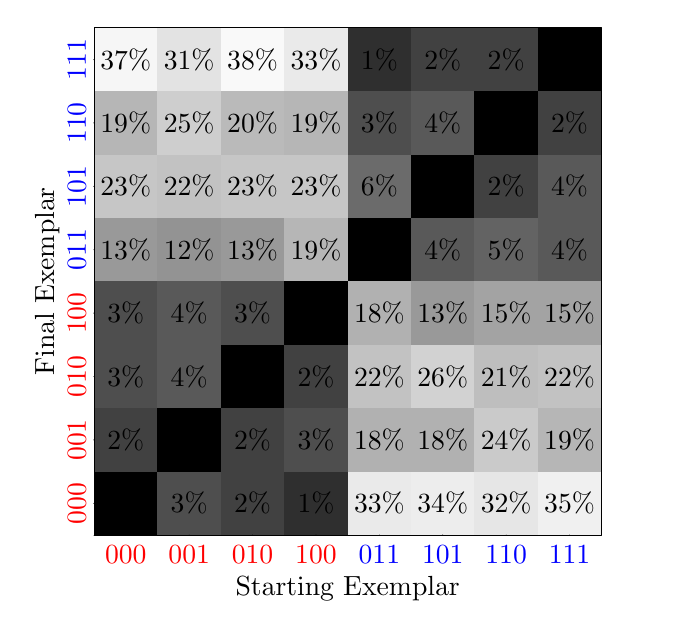
\begin{tikzpicture}[x=1pt,y=1pt]
\definecolor{fillColor}{RGB}{255,255,255}
\path[use as bounding box,fill=fillColor,fill opacity=0.00] (0,0) rectangle (231.26,207.41);
\begin{scope}
\path[clip] ( 24.00, 24.00) rectangle (207.26,207.41);
\definecolor{fillColor}{RGB}{0,0,0}

\path[fill=fillColor] ( 24.00, 24.08) rectangle ( 46.91, 46.98);
\definecolor{fillColor}{RGB}{65,65,65}

\path[fill=fillColor] ( 24.00, 46.98) rectangle ( 46.91, 69.89);
\definecolor{fillColor}{RGB}{78,78,78}

\path[fill=fillColor] ( 24.00, 69.89) rectangle ( 46.91, 92.80);

\path[fill=fillColor] ( 24.00, 92.80) rectangle ( 46.91,115.71);
\definecolor{fillColor}{gray}{0.60}

\path[fill=fillColor] ( 24.00,115.71) rectangle ( 46.91,138.62);
\definecolor{fillColor}{RGB}{198,198,198}

\path[fill=fillColor] ( 24.00,138.62) rectangle ( 46.91,161.52);
\definecolor{fillColor}{RGB}{182,182,182}

\path[fill=fillColor] ( 24.00,161.52) rectangle ( 46.91,184.43);
\definecolor{fillColor}{RGB}{246,246,246}

\path[fill=fillColor] ( 24.00,184.43) rectangle ( 46.91,207.34);
\definecolor{fillColor}{RGB}{78,78,78}

\path[fill=fillColor] ( 46.91, 24.08) rectangle ( 69.82, 46.98);
\definecolor{fillColor}{RGB}{0,0,0}

\path[fill=fillColor] ( 46.91, 46.98) rectangle ( 69.82, 69.89);
\definecolor{fillColor}{gray}{0.35}

\path[fill=fillColor] ( 46.91, 69.89) rectangle ( 69.82, 92.80);

\path[fill=fillColor] ( 46.91, 92.80) rectangle ( 69.82,115.71);
\definecolor{fillColor}{RGB}{147,147,147}

\path[fill=fillColor] ( 46.91,115.71) rectangle ( 69.82,138.62);
\definecolor{fillColor}{gray}{0.76}

\path[fill=fillColor] ( 46.91,138.62) rectangle ( 69.82,161.52);
\definecolor{fillColor}{RGB}{206,206,206}

\path[fill=fillColor] ( 46.91,161.52) rectangle ( 69.82,184.43);
\definecolor{fillColor}{gray}{0.89}

\path[fill=fillColor] ( 46.91,184.43) rectangle ( 69.82,207.34);
\definecolor{fillColor}{RGB}{65,65,65}

\path[fill=fillColor] ( 69.82, 24.08) rectangle ( 92.72, 46.98);

\path[fill=fillColor] ( 69.82, 46.98) rectangle ( 92.72, 69.89);
\definecolor{fillColor}{RGB}{0,0,0}

\path[fill=fillColor] ( 69.82, 69.89) rectangle ( 92.72, 92.80);
\definecolor{fillColor}{RGB}{78,78,78}

\path[fill=fillColor] ( 69.82, 92.80) rectangle ( 92.72,115.71);
\definecolor{fillColor}{gray}{0.60}

\path[fill=fillColor] ( 69.82,115.71) rectangle ( 92.72,138.62);
\definecolor{fillColor}{RGB}{198,198,198}

\path[fill=fillColor] ( 69.82,138.62) rectangle ( 92.72,161.52);
\definecolor{fillColor}{gray}{0.73}

\path[fill=fillColor] ( 69.82,161.52) rectangle ( 92.72,184.43);
\definecolor{fillColor}{RGB}{249,249,249}

\path[fill=fillColor] ( 69.82,184.43) rectangle ( 92.72,207.34);
\definecolor{fillColor}{RGB}{47,47,47}

\path[fill=fillColor] ( 92.72, 24.08) rectangle (115.63, 46.98);
\definecolor{fillColor}{RGB}{78,78,78}

\path[fill=fillColor] ( 92.72, 46.98) rectangle (115.63, 69.89);
\definecolor{fillColor}{RGB}{65,65,65}

\path[fill=fillColor] ( 92.72, 69.89) rectangle (115.63, 92.80);
\definecolor{fillColor}{RGB}{0,0,0}

\path[fill=fillColor] ( 92.72, 92.80) rectangle (115.63,115.71);
\definecolor{fillColor}{RGB}{182,182,182}

\path[fill=fillColor] ( 92.72,115.71) rectangle (115.63,138.62);
\definecolor{fillColor}{RGB}{198,198,198}

\path[fill=fillColor] ( 92.72,138.62) rectangle (115.63,161.52);
\definecolor{fillColor}{RGB}{182,182,182}

\path[fill=fillColor] ( 92.72,161.52) rectangle (115.63,184.43);
\definecolor{fillColor}{RGB}{234,234,234}

\path[fill=fillColor] ( 92.72,184.43) rectangle (115.63,207.34);

\path[fill=fillColor] (115.63, 24.08) rectangle (138.54, 46.98);
\definecolor{fillColor}{RGB}{177,177,177}

\path[fill=fillColor] (115.63, 46.98) rectangle (138.54, 69.89);
\definecolor{fillColor}{gray}{0.76}

\path[fill=fillColor] (115.63, 69.89) rectangle (138.54, 92.80);
\definecolor{fillColor}{RGB}{177,177,177}

\path[fill=fillColor] (115.63, 92.80) rectangle (138.54,115.71);
\definecolor{fillColor}{RGB}{0,0,0}

\path[fill=fillColor] (115.63,115.71) rectangle (138.54,138.62);
\definecolor{fillColor}{gray}{0.42}

\path[fill=fillColor] (115.63,138.62) rectangle (138.54,161.52);
\definecolor{fillColor}{RGB}{78,78,78}

\path[fill=fillColor] (115.63,161.52) rectangle (138.54,184.43);
\definecolor{fillColor}{RGB}{47,47,47}

\path[fill=fillColor] (115.63,184.43) rectangle (138.54,207.34);
\definecolor{fillColor}{gray}{0.93}

\path[fill=fillColor] (138.54, 24.08) rectangle (161.45, 46.98);
\definecolor{fillColor}{RGB}{177,177,177}

\path[fill=fillColor] (138.54, 46.98) rectangle (161.45, 69.89);
\definecolor{fillColor}{RGB}{210,210,210}

\path[fill=fillColor] (138.54, 69.89) rectangle (161.45, 92.80);
\definecolor{fillColor}{gray}{0.60}

\path[fill=fillColor] (138.54, 92.80) rectangle (161.45,115.71);
\definecolor{fillColor}{gray}{0.35}

\path[fill=fillColor] (138.54,115.71) rectangle (161.45,138.62);
\definecolor{fillColor}{RGB}{0,0,0}

\path[fill=fillColor] (138.54,138.62) rectangle (161.45,161.52);
\definecolor{fillColor}{gray}{0.35}

\path[fill=fillColor] (138.54,161.52) rectangle (161.45,184.43);
\definecolor{fillColor}{RGB}{65,65,65}

\path[fill=fillColor] (138.54,184.43) rectangle (161.45,207.34);
\definecolor{fillColor}{RGB}{230,230,230}

\path[fill=fillColor] (161.45, 24.08) rectangle (184.36, 46.98);
\definecolor{fillColor}{RGB}{202,202,202}

\path[fill=fillColor] (161.45, 46.98) rectangle (184.36, 69.89);
\definecolor{fillColor}{RGB}{190,190,190}

\path[fill=fillColor] (161.45, 69.89) rectangle (184.36, 92.80);
\definecolor{fillColor}{gray}{0.64}

\path[fill=fillColor] (161.45, 92.80) rectangle (184.36,115.71);
\definecolor{fillColor}{gray}{0.39}

\path[fill=fillColor] (161.45,115.71) rectangle (184.36,138.62);
\definecolor{fillColor}{RGB}{65,65,65}

\path[fill=fillColor] (161.45,138.62) rectangle (184.36,161.52);
\definecolor{fillColor}{RGB}{0,0,0}

\path[fill=fillColor] (161.45,161.52) rectangle (184.36,184.43);
\definecolor{fillColor}{RGB}{65,65,65}

\path[fill=fillColor] (161.45,184.43) rectangle (184.36,207.34);
\definecolor{fillColor}{gray}{0.94}

\path[fill=fillColor] (184.36, 24.08) rectangle (207.26, 46.98);
\definecolor{fillColor}{RGB}{182,182,182}

\path[fill=fillColor] (184.36, 46.98) rectangle (207.26, 69.89);
\definecolor{fillColor}{gray}{0.76}

\path[fill=fillColor] (184.36, 69.89) rectangle (207.26, 92.80);
\definecolor{fillColor}{gray}{0.64}

\path[fill=fillColor] (184.36, 92.80) rectangle (207.26,115.71);
\definecolor{fillColor}{gray}{0.35}

\path[fill=fillColor] (184.36,115.71) rectangle (207.26,138.62);

\path[fill=fillColor] (184.36,138.62) rectangle (207.26,161.52);
\definecolor{fillColor}{RGB}{65,65,65}

\path[fill=fillColor] (184.36,161.52) rectangle (207.26,184.43);
\definecolor{fillColor}{RGB}{0,0,0}

\path[fill=fillColor] (184.36,184.43) rectangle (207.26,207.34);
\end{scope}
\begin{scope}
\path[clip] (  0.00,  0.00) rectangle (231.26,207.41);
\definecolor{drawColor}{RGB}{0,0,0}

\node[text=drawColor,anchor=base,inner sep=0pt, outer sep=0pt, scale=  1.00] at (115.63,  2.40) {Starting Exemplar};

\node[text=drawColor,rotate= 90.00,anchor=base,inner sep=0pt, outer sep=0pt, scale=  1.00] at (  9.60,115.71) {Final Exemplar};
\end{scope}
\begin{scope}
\path[clip] (  0.00,  0.00) rectangle (231.26,207.41);
\definecolor{drawColor}{RGB}{0,0,0}

\path[draw=drawColor,line width= 0.4pt,line join=round,line cap=round] ( 35.45, 24.00) -- ( 35.45, 24.00);

\path[draw=drawColor,line width= 0.4pt,line join=round,line cap=round] ( 35.45, 24.00) -- ( 35.45, 24.00);
\definecolor{drawColor}{RGB}{255,0,0}

\node[text=drawColor,anchor=base,inner sep=0pt, outer sep=0pt, scale=  1.00] at ( 35.45, 13.80) {000};
\definecolor{drawColor}{RGB}{0,0,0}

\path[draw=drawColor,line width= 0.4pt,line join=round,line cap=round] ( 24.00, 35.53) -- ( 24.00, 35.53);

\path[draw=drawColor,line width= 0.4pt,line join=round,line cap=round] ( 24.00, 35.53) -- ( 24.00, 35.53);
\definecolor{drawColor}{RGB}{255,0,0}

\node[text=drawColor,rotate= 90.00,anchor=base,inner sep=0pt, outer sep=0pt, scale=  1.00] at ( 21.00, 35.53) {000};
\end{scope}
\begin{scope}
\path[clip] ( 24.00, 24.00) rectangle (207.26,207.41);
\definecolor{drawColor}{RGB}{0,0,0}

\node[text=drawColor,anchor=base,inner sep=0pt, outer sep=0pt, scale=  1.00] at ( 35.45, 54.97) {2{\%}};

\node[text=drawColor,anchor=base,inner sep=0pt, outer sep=0pt, scale=  1.00] at ( 35.45, 77.87) {3{\%}};

\node[text=drawColor,anchor=base,inner sep=0pt, outer sep=0pt, scale=  1.00] at ( 35.45,100.78) {3{\%}};

\node[text=drawColor,anchor=base,inner sep=0pt, outer sep=0pt, scale=  1.00] at ( 35.45,123.69) {13{\%}};

\node[text=drawColor,anchor=base,inner sep=0pt, outer sep=0pt, scale=  1.00] at ( 35.45,146.60) {23{\%}};

\node[text=drawColor,anchor=base,inner sep=0pt, outer sep=0pt, scale=  1.00] at ( 35.45,169.51) {19{\%}};

\node[text=drawColor,anchor=base,inner sep=0pt, outer sep=0pt, scale=  1.00] at ( 35.45,192.41) {37{\%}};
\end{scope}
\begin{scope}
\path[clip] (  0.00,  0.00) rectangle (231.26,207.41);
\definecolor{drawColor}{RGB}{0,0,0}

\path[draw=drawColor,line width= 0.4pt,line join=round,line cap=round] ( 58.36, 24.00) -- ( 58.36, 24.00);

\path[draw=drawColor,line width= 0.4pt,line join=round,line cap=round] ( 58.36, 24.00) -- ( 58.36, 24.00);
\definecolor{drawColor}{RGB}{255,0,0}

\node[text=drawColor,anchor=base,inner sep=0pt, outer sep=0pt, scale=  1.00] at ( 58.36, 13.80) {001};
\definecolor{drawColor}{RGB}{0,0,0}

\path[draw=drawColor,line width= 0.4pt,line join=round,line cap=round] ( 24.00, 58.44) -- ( 24.00, 58.44);

\path[draw=drawColor,line width= 0.4pt,line join=round,line cap=round] ( 24.00, 58.44) -- ( 24.00, 58.44);
\definecolor{drawColor}{RGB}{255,0,0}

\node[text=drawColor,rotate= 90.00,anchor=base,inner sep=0pt, outer sep=0pt, scale=  1.00] at ( 21.00, 58.44) {001};
\end{scope}
\begin{scope}
\path[clip] ( 24.00, 24.00) rectangle (207.26,207.41);
\definecolor{drawColor}{RGB}{0,0,0}

\node[text=drawColor,anchor=base,inner sep=0pt, outer sep=0pt, scale=  1.00] at ( 58.36, 32.06) {3{\%}};

\node[text=drawColor,anchor=base,inner sep=0pt, outer sep=0pt, scale=  1.00] at ( 58.36, 77.87) {4{\%}};

\node[text=drawColor,anchor=base,inner sep=0pt, outer sep=0pt, scale=  1.00] at ( 58.36,100.78) {4{\%}};

\node[text=drawColor,anchor=base,inner sep=0pt, outer sep=0pt, scale=  1.00] at ( 58.36,123.69) {12{\%}};

\node[text=drawColor,anchor=base,inner sep=0pt, outer sep=0pt, scale=  1.00] at ( 58.36,146.60) {22{\%}};

\node[text=drawColor,anchor=base,inner sep=0pt, outer sep=0pt, scale=  1.00] at ( 58.36,169.51) {25{\%}};

\node[text=drawColor,anchor=base,inner sep=0pt, outer sep=0pt, scale=  1.00] at ( 58.36,192.41) {31{\%}};
\end{scope}
\begin{scope}
\path[clip] (  0.00,  0.00) rectangle (231.26,207.41);
\definecolor{drawColor}{RGB}{0,0,0}

\path[draw=drawColor,line width= 0.4pt,line join=round,line cap=round] ( 81.27, 24.00) -- ( 81.27, 24.00);

\path[draw=drawColor,line width= 0.4pt,line join=round,line cap=round] ( 81.27, 24.00) -- ( 81.27, 24.00);
\definecolor{drawColor}{RGB}{255,0,0}

\node[text=drawColor,anchor=base,inner sep=0pt, outer sep=0pt, scale=  1.00] at ( 81.27, 13.80) {010};
\definecolor{drawColor}{RGB}{0,0,0}

\path[draw=drawColor,line width= 0.4pt,line join=round,line cap=round] ( 24.00, 81.35) -- ( 24.00, 81.35);

\path[draw=drawColor,line width= 0.4pt,line join=round,line cap=round] ( 24.00, 81.35) -- ( 24.00, 81.35);
\definecolor{drawColor}{RGB}{255,0,0}

\node[text=drawColor,rotate= 90.00,anchor=base,inner sep=0pt, outer sep=0pt, scale=  1.00] at ( 21.00, 81.35) {010};
\end{scope}
\begin{scope}
\path[clip] ( 24.00, 24.00) rectangle (207.26,207.41);
\definecolor{drawColor}{RGB}{0,0,0}

\node[text=drawColor,anchor=base,inner sep=0pt, outer sep=0pt, scale=  1.00] at ( 81.27, 32.06) {2{\%}};

\node[text=drawColor,anchor=base,inner sep=0pt, outer sep=0pt, scale=  1.00] at ( 81.27, 54.97) {2{\%}};

\node[text=drawColor,anchor=base,inner sep=0pt, outer sep=0pt, scale=  1.00] at ( 81.27,100.78) {3{\%}};

\node[text=drawColor,anchor=base,inner sep=0pt, outer sep=0pt, scale=  1.00] at ( 81.27,123.69) {13{\%}};

\node[text=drawColor,anchor=base,inner sep=0pt, outer sep=0pt, scale=  1.00] at ( 81.27,146.60) {23{\%}};

\node[text=drawColor,anchor=base,inner sep=0pt, outer sep=0pt, scale=  1.00] at ( 81.27,169.51) {20{\%}};

\node[text=drawColor,anchor=base,inner sep=0pt, outer sep=0pt, scale=  1.00] at ( 81.27,192.41) {38{\%}};
\end{scope}
\begin{scope}
\path[clip] (  0.00,  0.00) rectangle (231.26,207.41);
\definecolor{drawColor}{RGB}{0,0,0}

\path[draw=drawColor,line width= 0.4pt,line join=round,line cap=round] (104.18, 24.00) -- (104.18, 24.00);

\path[draw=drawColor,line width= 0.4pt,line join=round,line cap=round] (104.18, 24.00) -- (104.18, 24.00);
\definecolor{drawColor}{RGB}{255,0,0}

\node[text=drawColor,anchor=base,inner sep=0pt, outer sep=0pt, scale=  1.00] at (104.18, 13.80) {100};
\definecolor{drawColor}{RGB}{0,0,0}

\path[draw=drawColor,line width= 0.4pt,line join=round,line cap=round] ( 24.00,104.25) -- ( 24.00,104.25);

\path[draw=drawColor,line width= 0.4pt,line join=round,line cap=round] ( 24.00,104.25) -- ( 24.00,104.25);
\definecolor{drawColor}{RGB}{255,0,0}

\node[text=drawColor,rotate= 90.00,anchor=base,inner sep=0pt, outer sep=0pt, scale=  1.00] at ( 21.00,104.25) {100};
\end{scope}
\begin{scope}
\path[clip] ( 24.00, 24.00) rectangle (207.26,207.41);
\definecolor{drawColor}{RGB}{0,0,0}

\node[text=drawColor,anchor=base,inner sep=0pt, outer sep=0pt, scale=  1.00] at (104.18, 32.06) {1{\%}};

\node[text=drawColor,anchor=base,inner sep=0pt, outer sep=0pt, scale=  1.00] at (104.18, 54.97) {3{\%}};

\node[text=drawColor,anchor=base,inner sep=0pt, outer sep=0pt, scale=  1.00] at (104.18, 77.87) {2{\%}};

\node[text=drawColor,anchor=base,inner sep=0pt, outer sep=0pt, scale=  1.00] at (104.18,123.69) {19{\%}};

\node[text=drawColor,anchor=base,inner sep=0pt, outer sep=0pt, scale=  1.00] at (104.18,146.60) {23{\%}};

\node[text=drawColor,anchor=base,inner sep=0pt, outer sep=0pt, scale=  1.00] at (104.18,169.51) {19{\%}};

\node[text=drawColor,anchor=base,inner sep=0pt, outer sep=0pt, scale=  1.00] at (104.18,192.41) {33{\%}};
\end{scope}
\begin{scope}
\path[clip] (  0.00,  0.00) rectangle (231.26,207.41);
\definecolor{drawColor}{RGB}{0,0,0}

\path[draw=drawColor,line width= 0.4pt,line join=round,line cap=round] (127.09, 24.00) -- (127.09, 24.00);

\path[draw=drawColor,line width= 0.4pt,line join=round,line cap=round] (127.09, 24.00) -- (127.09, 24.00);
\definecolor{drawColor}{RGB}{0,0,255}

\node[text=drawColor,anchor=base,inner sep=0pt, outer sep=0pt, scale=  1.00] at (127.09, 13.80) {011};
\definecolor{drawColor}{RGB}{0,0,0}

\path[draw=drawColor,line width= 0.4pt,line join=round,line cap=round] ( 24.00,127.16) -- ( 24.00,127.16);

\path[draw=drawColor,line width= 0.4pt,line join=round,line cap=round] ( 24.00,127.16) -- ( 24.00,127.16);
\definecolor{drawColor}{RGB}{0,0,255}

\node[text=drawColor,rotate= 90.00,anchor=base,inner sep=0pt, outer sep=0pt, scale=  1.00] at ( 21.00,127.16) {011};
\end{scope}
\begin{scope}
\path[clip] ( 24.00, 24.00) rectangle (207.26,207.41);
\definecolor{drawColor}{RGB}{0,0,0}

\node[text=drawColor,anchor=base,inner sep=0pt, outer sep=0pt, scale=  1.00] at (127.09, 32.06) {33{\%}};

\node[text=drawColor,anchor=base,inner sep=0pt, outer sep=0pt, scale=  1.00] at (127.09, 54.97) {18{\%}};

\node[text=drawColor,anchor=base,inner sep=0pt, outer sep=0pt, scale=  1.00] at (127.09, 77.87) {22{\%}};

\node[text=drawColor,anchor=base,inner sep=0pt, outer sep=0pt, scale=  1.00] at (127.09,100.78) {18{\%}};

\node[text=drawColor,anchor=base,inner sep=0pt, outer sep=0pt, scale=  1.00] at (127.09,146.60) {6{\%}};

\node[text=drawColor,anchor=base,inner sep=0pt, outer sep=0pt, scale=  1.00] at (127.09,169.51) {3{\%}};

\node[text=drawColor,anchor=base,inner sep=0pt, outer sep=0pt, scale=  1.00] at (127.09,192.41) {1{\%}};
\end{scope}
\begin{scope}
\path[clip] (  0.00,  0.00) rectangle (231.26,207.41);
\definecolor{drawColor}{RGB}{0,0,0}

\path[draw=drawColor,line width= 0.4pt,line join=round,line cap=round] (149.99, 24.00) -- (149.99, 24.00);

\path[draw=drawColor,line width= 0.4pt,line join=round,line cap=round] (149.99, 24.00) -- (149.99, 24.00);
\definecolor{drawColor}{RGB}{0,0,255}

\node[text=drawColor,anchor=base,inner sep=0pt, outer sep=0pt, scale=  1.00] at (149.99, 13.80) {101};
\definecolor{drawColor}{RGB}{0,0,0}

\path[draw=drawColor,line width= 0.4pt,line join=round,line cap=round] ( 24.00,150.07) -- ( 24.00,150.07);

\path[draw=drawColor,line width= 0.4pt,line join=round,line cap=round] ( 24.00,150.07) -- ( 24.00,150.07);
\definecolor{drawColor}{RGB}{0,0,255}

\node[text=drawColor,rotate= 90.00,anchor=base,inner sep=0pt, outer sep=0pt, scale=  1.00] at ( 21.00,150.07) {101};
\end{scope}
\begin{scope}
\path[clip] ( 24.00, 24.00) rectangle (207.26,207.41);
\definecolor{drawColor}{RGB}{0,0,0}

\node[text=drawColor,anchor=base,inner sep=0pt, outer sep=0pt, scale=  1.00] at (149.99, 32.06) {34{\%}};

\node[text=drawColor,anchor=base,inner sep=0pt, outer sep=0pt, scale=  1.00] at (149.99, 54.97) {18{\%}};

\node[text=drawColor,anchor=base,inner sep=0pt, outer sep=0pt, scale=  1.00] at (149.99, 77.87) {26{\%}};

\node[text=drawColor,anchor=base,inner sep=0pt, outer sep=0pt, scale=  1.00] at (149.99,100.78) {13{\%}};

\node[text=drawColor,anchor=base,inner sep=0pt, outer sep=0pt, scale=  1.00] at (149.99,123.69) {4{\%}};

\node[text=drawColor,anchor=base,inner sep=0pt, outer sep=0pt, scale=  1.00] at (149.99,169.51) {4{\%}};

\node[text=drawColor,anchor=base,inner sep=0pt, outer sep=0pt, scale=  1.00] at (149.99,192.41) {2{\%}};
\end{scope}
\begin{scope}
\path[clip] (  0.00,  0.00) rectangle (231.26,207.41);
\definecolor{drawColor}{RGB}{0,0,0}

\path[draw=drawColor,line width= 0.4pt,line join=round,line cap=round] (172.90, 24.00) -- (172.90, 24.00);

\path[draw=drawColor,line width= 0.4pt,line join=round,line cap=round] (172.90, 24.00) -- (172.90, 24.00);
\definecolor{drawColor}{RGB}{0,0,255}

\node[text=drawColor,anchor=base,inner sep=0pt, outer sep=0pt, scale=  1.00] at (172.90, 13.80) {110};
\definecolor{drawColor}{RGB}{0,0,0}

\path[draw=drawColor,line width= 0.4pt,line join=round,line cap=round] ( 24.00,172.98) -- ( 24.00,172.98);

\path[draw=drawColor,line width= 0.4pt,line join=round,line cap=round] ( 24.00,172.98) -- ( 24.00,172.98);
\definecolor{drawColor}{RGB}{0,0,255}

\node[text=drawColor,rotate= 90.00,anchor=base,inner sep=0pt, outer sep=0pt, scale=  1.00] at ( 21.00,172.98) {110};
\end{scope}
\begin{scope}
\path[clip] ( 24.00, 24.00) rectangle (207.26,207.41);
\definecolor{drawColor}{RGB}{0,0,0}

\node[text=drawColor,anchor=base,inner sep=0pt, outer sep=0pt, scale=  1.00] at (172.90, 32.06) {32{\%}};

\node[text=drawColor,anchor=base,inner sep=0pt, outer sep=0pt, scale=  1.00] at (172.90, 54.97) {24{\%}};

\node[text=drawColor,anchor=base,inner sep=0pt, outer sep=0pt, scale=  1.00] at (172.90, 77.87) {21{\%}};

\node[text=drawColor,anchor=base,inner sep=0pt, outer sep=0pt, scale=  1.00] at (172.90,100.78) {15{\%}};

\node[text=drawColor,anchor=base,inner sep=0pt, outer sep=0pt, scale=  1.00] at (172.90,123.69) {5{\%}};

\node[text=drawColor,anchor=base,inner sep=0pt, outer sep=0pt, scale=  1.00] at (172.90,146.60) {2{\%}};

\node[text=drawColor,anchor=base,inner sep=0pt, outer sep=0pt, scale=  1.00] at (172.90,192.41) {2{\%}};
\end{scope}
\begin{scope}
\path[clip] (  0.00,  0.00) rectangle (231.26,207.41);
\definecolor{drawColor}{RGB}{0,0,0}

\path[draw=drawColor,line width= 0.4pt,line join=round,line cap=round] (195.81, 24.00) -- (195.81, 24.00);

\path[draw=drawColor,line width= 0.4pt,line join=round,line cap=round] (195.81, 24.00) -- (195.81, 24.00);
\definecolor{drawColor}{RGB}{0,0,255}

\node[text=drawColor,anchor=base,inner sep=0pt, outer sep=0pt, scale=  1.00] at (195.81, 13.80) {111};
\definecolor{drawColor}{RGB}{0,0,0}

\path[draw=drawColor,line width= 0.4pt,line join=round,line cap=round] ( 24.00,195.89) -- ( 24.00,195.89);

\path[draw=drawColor,line width= 0.4pt,line join=round,line cap=round] ( 24.00,195.89) -- ( 24.00,195.89);
\definecolor{drawColor}{RGB}{0,0,255}

\node[text=drawColor,rotate= 90.00,anchor=base,inner sep=0pt, outer sep=0pt, scale=  1.00] at ( 21.00,195.89) {111};
\end{scope}
\begin{scope}
\path[clip] ( 24.00, 24.00) rectangle (207.26,207.41);
\definecolor{drawColor}{RGB}{0,0,0}

\node[text=drawColor,anchor=base,inner sep=0pt, outer sep=0pt, scale=  1.00] at (195.81, 32.06) {35{\%}};

\node[text=drawColor,anchor=base,inner sep=0pt, outer sep=0pt, scale=  1.00] at (195.81, 54.97) {19{\%}};

\node[text=drawColor,anchor=base,inner sep=0pt, outer sep=0pt, scale=  1.00] at (195.81, 77.87) {22{\%}};

\node[text=drawColor,anchor=base,inner sep=0pt, outer sep=0pt, scale=  1.00] at (195.81,100.78) {15{\%}};

\node[text=drawColor,anchor=base,inner sep=0pt, outer sep=0pt, scale=  1.00] at (195.81,123.69) {4{\%}};

\node[text=drawColor,anchor=base,inner sep=0pt, outer sep=0pt, scale=  1.00] at (195.81,146.60) {4{\%}};

\node[text=drawColor,anchor=base,inner sep=0pt, outer sep=0pt, scale=  1.00] at (195.81,169.51) {2{\%}};
\end{scope}
\begin{scope}
\path[clip] (  0.00,  0.00) rectangle (231.26,207.41);
\definecolor{drawColor}{RGB}{0,0,0}

\path[draw=drawColor,line width= 0.4pt,line join=round,line cap=round] ( 24.00, 24.00) --
	(207.26, 24.00) --
	(207.26,207.41) --
	( 24.00,207.41) --
	( 24.00, 24.00);
\end{scope}
\end{tikzpicture}
